\begin{tikzpicture}[font=\sffamily\fontsize{10}{9}\selectfont]
    \def\RFILE{Figures/plotdata/irat.csv}
    \def\RFILE{..//paper_data_v3/irat_enet/final_irat_model/results/irat1.csv}
  \def\WDT{6.25in}
  \def\HGT{4.35in}
  \def\WDTs{1.6in}
  \def\HGTs{1.6in}
  \def\OPC{.2}
  \def\XFT{-.765in}
\def\TEXTCOLA{black!50}
\def\MCOL{DodgerBlue4!60}
\def\COLBLUE{DodgerBlue3}
\def\DCOL{black!20}
\def\TXTSZ{6}
\def\GGCOL{black!15}
      \def\FCOL{DarkOrange1!50}
      \def\FCOLA{DarkOrange2!50}
  \def\AXISCOL{black!15}

\clip (-3.8in,-5.3in) rectangle (3in,2.75in);

  
  \coordinate (Z) at (0,0);
    \node[] (A) at (Z) {
  \begin{tikzpicture}[anchor=center]
   \pgfplotsset{
    discard if/.style 2 args={
      x filter/.append code={
        \edef\tempa{\thisrow{#1}}
        \edef\tempb{#2}
        \ifx\tempa\tempb
        \def\pgfmathresult{inf}
        \fi
      }
    },
    discard if not/.style 2 args={
      x filter/.append code={
        \edef\tempa{\thisrow{#1}}
        \edef\tempb{#2}
        \ifx\tempa\tempb
        \else
        \def\pgfmathresult{inf}
        \fi
      }
    },
    % define the style of the `nodes near coords' that should be shown
    % above the point
    nodes near coords above style/.style={
      font=\bf\fontsize{\TXTSZ}{5}\selectfont,
      text=\TEXTCOLA,
      nodes near coords style={
        anchor=south west,yshift=.070in,
      },
    },
    % define the style of the `nodes near coords' that should be shown
    % above the point
    nodes near coords axove style/.style={
      font=\bf\fontsize{\TXTSZ}{5}\selectfont,
      text=\TEXTCOLA,
      nodes near coords style={
        anchor=south east,yshift=.02in,
      },
    },
    % define the style of the `nodes near coords' that should be shown
    % above the point
    nodes near coords belox style/.style={
      font=\bf\fontsize{\TXTSZ}{5}\selectfont,
      text=\TEXTCOLA,
      nodes near coords style={
        anchor=north west,yshift=.0in,
      },
    },
    % define the style of the `nodes near coords' that should be shown
    % above the point
    nodes near coords beloxx style/.style={
      font=\bf\fontsize{\TXTSZ}{5}\selectfont,
      text=\TEXTCOLA,
      nodes near coords style={
        anchor=north west,yshift=.02in,
      },
    },
    % define the style of the `nodes near coords' that should be shown
    % below the point
    nodes near coords below style/.style={
       font=\bf\fontsize{\TXTSZ}{5}\selectfont,
      text=\TEXTCOLA,
     nodes near coords style={
        anchor=north, yshift=-.05in, xshift=-.1in,
      },
    },
    % define the style of the `nodes near coords' that should be shown
    % below the point
    nodes near coords right style/.style={
        font=\bf\fontsize{\TXTSZ}{5}\selectfont,
      text=\TEXTCOLA,
    nodes near coords style={
        anchor=west,xshift=0.02in,
      },
    },
    % define the style of the `nodes near coords' that should be shown
    % below the point
    nodes near coords left style/.style={
       font=\bf\fontsize{\TXTSZ}{5}\selectfont,
       text=\TEXTCOLA,
    nodes near coords style={
        anchor=east,
        xshift=-.02in,yshift=-.04in,
      },
    },
    % define the style of the `nodes near coords' that should be shown
    % below the point
    nodes near coords null style/.style={
         font=\bf\fontsize{\TXTSZ}{5}\selectfont,
      text=\TEXTCOLA,
   nodes near coords style={
        anchor=west,text opacity=0,
      },
    },
  }
    \begin{axis}[enlargelimits=false,scale only axis=true,
      axis line style={\AXISCOL, opacity=1,thin, rounded corners=0pt},
      grid style={thin,\GGCOL},
      grid=both,
      enlargelimits=false, 
      width=\WDT, 
      height=\HGT,
      scaled ticks = false,
      x tick label style={yshift=-.05in,/pgf/number format/fixed,
        /pgf/number format/1000 sep = %\thinspace % Optional if you want to replace comma as the 1000 separator 
      },yticklabel style={/pgf/number format/fixed,
        /pgf/number format/precision=2},,xticklabel style={/pgf/number format/fixed,
        /pgf/number format/precision=2},
      major tick length=0pt,
      yticklabel style={xshift=-.015in}, nodes near coords,
      point meta=explicit symbolic,
      table/meta=Influenza Virus,      axis on top=false,
      xlabel={negative logarithm of geometric mean of HA and NA \qdist },ylabel={CDC computed IRAT emergence score},xlabel style={yshift=-.1in},ylabel style={yshift=-.12in},ymin=2.5,xmax=7.75,xmin=1.75,
      ]

      % \addplot[smooth, ultra thick,draw=none, opacity=1,mark=*,
      % nodes near coords null style, ] table[col sep=comma,columns/Influenza Virus/.style={string type},
      % x=logrisk,y=Emergence Score] \RFILE;
      % \addplot[smooth, ultra thick,draw=black, opacity=1,mark=none,
      % nodes near coords null style, ] table[col sep=comma,columns/Influenza Virus/.style={string type},
      % x=logrisk,y=pred_GM] \RFILE;


      \addplot[smooth, ultra thick,draw=white, opacity=1,mark=none,
      nodes near coords null style, ] table[col sep=comma,
      x=logrisk,y=pred_GM] \RFILE;

      \addplot[nodes near coords null style,forget plot,
      name path=UB,smooth, ultra thick,
      mark=none,draw=none ] table[col sep=comma,
      x=logrisk,y=ub_GM] \RFILE;
      
      \addplot[nodes near coords null style,
      forget plot, name path=LB,smooth,
      ultra thick, mark=none,draw=none ] table[col sep=comma,
      x=logrisk,y=lb_GM] \RFILE;
      
      \addplot[nodes near coords null style,
      forget plot,\FCOLA,opacity=1] fill between[of=LB and UB];
      
     
      \addplot[only marks, mark=*,
      mark options={fill=black,fill=\MCOL,draw=\DCOL,scale=1.5},
      nodes near coords below style,      
      discard if={Influenza Virus}{A/Shanghai/02/2013},
      discard if={Influenza Virus}{A/Indiana/08/2011},
      discard if={Influenza Virus}{A/Ohio/13/2017},
      discard if={Influenza Virus}{A/Hong Kong/125/2017},
      discard if={Influenza Virus}{A/Sichuan/06681/2021},
      discard if={Influenza Virus}{A/California/62/2018},
      discard if={Influenza Virus}{A/Bangladesh/0994/2011},
      discard if={Influenza Virus}{A/Anhui-Lujiang/39/2018},
      discard if={Influenza Virus}{A/chicken/Tennessee/17-007431-3/2017},
      discard if={Influenza Virus}{A/chicken/Tennessee/17-007147-2/2017},
      discard if={Influenza Virus}{A/Yunnan/14564/2015},
      discard if={Influenza Virus}{A/Astrakhan/3212/2020},
      discard if={Influenza Virus}{A/canine/Illinois/12191/2015},
      discard if={Influenza Virus}{A/gyrfalcon/Washington/41088/2014},
      discard if={Influenza Virus}{A/turkey/Indiana/1573-2/2016},
      discard if={Influenza Virus}{A/American wigeon/South Carolina/AH0195145/2021},
      discard if={Influenza Virus}{A/Jiangxi-Donghu/346/2013},
      %discard if={Influenza Virus}{A/swine/Shandong/1207/2016},
      discard if={Influenza Virus}{A/American green-winged teal/Washington/1957050/2014},
      discard if={Influenza Virus}{A/Northern pintail/Washington/40964/2014},
      discard if={Influenza Virus}{A/Netherlands/219/2003} ]
      table[x=logrisk,
      y=Emergence Score,col sep=comma] \RFILE;


      \pgfplotsinvokeforeach {
         A/Northern pintail/Washington/40964/2014,
       A/Netherlands/219/2003%
      } {
        \addplot+ [only marks,
        mark=*,
        mark options={fill=\MCOL,draw=\DCOL,scale=1.5},
        nodes near coords below style,
        forget plot,text=black,
        nodes near coords above style,
        discard if not={Influenza Virus}{#1},
        ] table[x=logrisk,
        y=Emergence Score,col sep=comma]\RFILE;
      }


      \pgfplotsinvokeforeach {
        A/Jiangxi-Donghu/346/2013,
        A/turkey/Indiana/1573-2/2016,
        A/American green-winged teal/Washington/1957050/2014,
        A/chicken/Tennessee/17-007147-2/2017,
        A/American wigeon/South Carolina/AH0195145/2021,
        A/chicken/Tennessee/17-007431-3/2017,A/Astrakhan/3212/2020,
        A/Yunnan/14564/2015%
      } {
        \addplot+ [only marks,
        mark=*,mark options={fill=black,fill=\MCOL,draw=\DCOL,scale=1.5},
        forget plot,
        nodes near coords right style,
        discard if not={Influenza Virus}{#1},
        ] table[x=logrisk,
        y=Emergence Score,col sep=comma]\RFILE;
      }

      \pgfplotsinvokeforeach {
       % A/swine/Shandong/1207/2016,
        A/canine/Illinois/12191/2015,
        A/Indiana/08/2011,
        A/Shanghai/02/2013,
        A/Hong Kong/125/2017,
        A/Sichuan/06681/2021,
        A/Bangladesh/0994/2011,
        A/Anhui-Lujiang/39/2018,
        A/California/62/2018% 
      } {
        \addplot+ [only marks,
        mark=*,mark options={fill=black,fill=\MCOL,draw=\DCOL,scale=1.50},
        forget plot,
        nodes near coords left style,
        discard if not={Influenza Virus}{#1},
        ] table[x=logrisk,
        y=Emergence Score,col sep=comma]\RFILE;
      }

      \pgfplotsinvokeforeach {
        A/Ohio/13/2017,
      } {
        \addplot+ [only marks,
        mark=*,mark options={fill=black,fill=\MCOL,draw=\DCOL,scale=1.50},
        forget plot,
        nodes near coords axove style,
        discard if not={Influenza Virus}{#1},
        ] table[x=logrisk,
        y=Emergence Score,col sep=comma]\RFILE;
      }

     \pgfplotsinvokeforeach {
 A/gyrfalcon/Washington/41088/2014,
      } {
        \addplot+ [only marks,
        mark=*,mark options={fill=black,fill=\MCOL,draw=\DCOL,scale=1.50},
        forget plot,
        nodes near coords belox style,
        discard if not={Influenza Virus}{#1},
        ] table[x=logrisk,
        y=Emergence Score,col sep=comma]\RFILE;
      }
     % \pgfplotsinvokeforeach {A/Jiangxi-Donghu/346/2013,
     %  } {
     %    \addplot+ [only marks,
     %    mark=*,mark options={fill=black,fill=\MCOL,draw=\DCOL,scale=1.50},
     %    forget plot,
     %    nodes near coords beloxx style,
     %    discard if not={Influenza Virus}{#1},
     %    ] table[x=logrisk,
     %    y=Emergence Score,col sep=comma]\RFILE;
     %  }

      \node [anchor=center,font=\bf\sffamily\fontsize{6}{6}\selectfont] at (axis cs:2.5,3) {H7N9};
      \node [anchor=center,font=\bf\sffamily\fontsize{6}{6}\selectfont] at (axis cs:2.9,3.265) {H7N9};
  \node [anchor=center,font=\bf\sffamily\fontsize{6}{6}\selectfont] at (axis cs:5,5.2) {H5N6};
  \node [anchor=center,font=\bf\sffamily\fontsize{6}{6}\selectfont] at (axis cs:2.5,4.4) {H10N8};
 \node [anchor=center,font=\bf\sffamily\fontsize{6}{6}\selectfont] at (axis cs:2.75,4.15) {H5N8};
  \node [anchor=center,font=\bf\sffamily\fontsize{6}{6}\selectfont] at (axis cs:2.4,3.27) {H7N8};
   \node [anchor=center,font=\bf\sffamily\fontsize{6}{6}\selectfont] at (axis cs:4.25,3.45) {H5N1};
  \node [anchor=center,font=\bf\sffamily\fontsize{6}{6}\selectfont] at (axis cs:3.9,3.8) {H5N2};
 \node [anchor=center,font=\bf\sffamily\fontsize{6}{6}\selectfont] at (axis cs:2,4.8) {H7N7};
   \node [anchor=center,font=\bf\sffamily\fontsize{6}{6}\selectfont] at (axis cs:4.4,3.8) {H5N8};
      \node [anchor=center,font=\bf\sffamily\fontsize{6}{6}\selectfont] at (axis cs:5,4.3) {H10N8};
      \node [anchor=center,font=\bf\sffamily\fontsize{6}{6}\selectfont] at (axis cs:5.7,6) {H9N2};
      \node [anchor=center,font=\bf\sffamily\fontsize{6}{6}\selectfont] at (axis cs:5.7,5.4) {H5N6};
      \node [anchor=center,font=\bf\sffamily\fontsize{6}{6}\selectfont] at (axis cs:6,6.8) {H3N2};
      \node [anchor=center,font=\bf\sffamily\fontsize{6}{6}\selectfont] at (axis cs:7.25,5.87) {H3N2};
      \node [anchor=center,font=\bf\sffamily\fontsize{6}{6}\selectfont] at (axis cs:6,5.1) {H5N1};
      \node [anchor=center,font=\bf\sffamily\fontsize{6}{6}\selectfont] at (axis cs:5.7,7.2) {H1N1};
 \node [anchor=center,font=\bf\sffamily\fontsize{6}{6}\selectfont] at (axis cs:2.05,4.45) {H5N8};
      \node [anchor=center,font=\bf\sffamily\fontsize{6}{6}\selectfont] at (axis cs:5.7,4.8) {H5N1};
      \node [anchor=center,font=\bf\sffamily\fontsize{6}{6}\selectfont] at (axis cs:7.25,6.55) {H7N9};
      \node [anchor=center,font=\bf\sffamily\fontsize{6}{6}\selectfont] at (axis cs:7.25,6.25) {H7N9};
      \node [anchor=center,font=\bf\sffamily\fontsize{6}{6}\selectfont] at (axis cs:7.25,5.65) {H1N2};


            \node [text=\COLBLUE,anchor=north west,fill=lightgray!20, fill opacity=.5, inner sep=6pt, rounded corners=5pt,,align=left,font=\bf\sffamily\fontsize{8}{9}\selectfont] (LLEQ1) at (axis cs:2,6.5) {Regression Eqn: $y = 0.47x + 2.77$\\$R = 0.72$\\p-value: $0.0001$};

            
    \end{axis}
  \end{tikzpicture}};


  \node[anchor=north west] (W) at ([yshift=-.4in]A.south west) {
    \begin{tikzpicture}[font=\bf\sffamily\fontsize{8}{8}\selectfont]
 \begin{scope}
 \clip (-3.4in,1.25in) rectangle (3.35in,-1in);
\node[anchor=center] (A11) at (0,0) {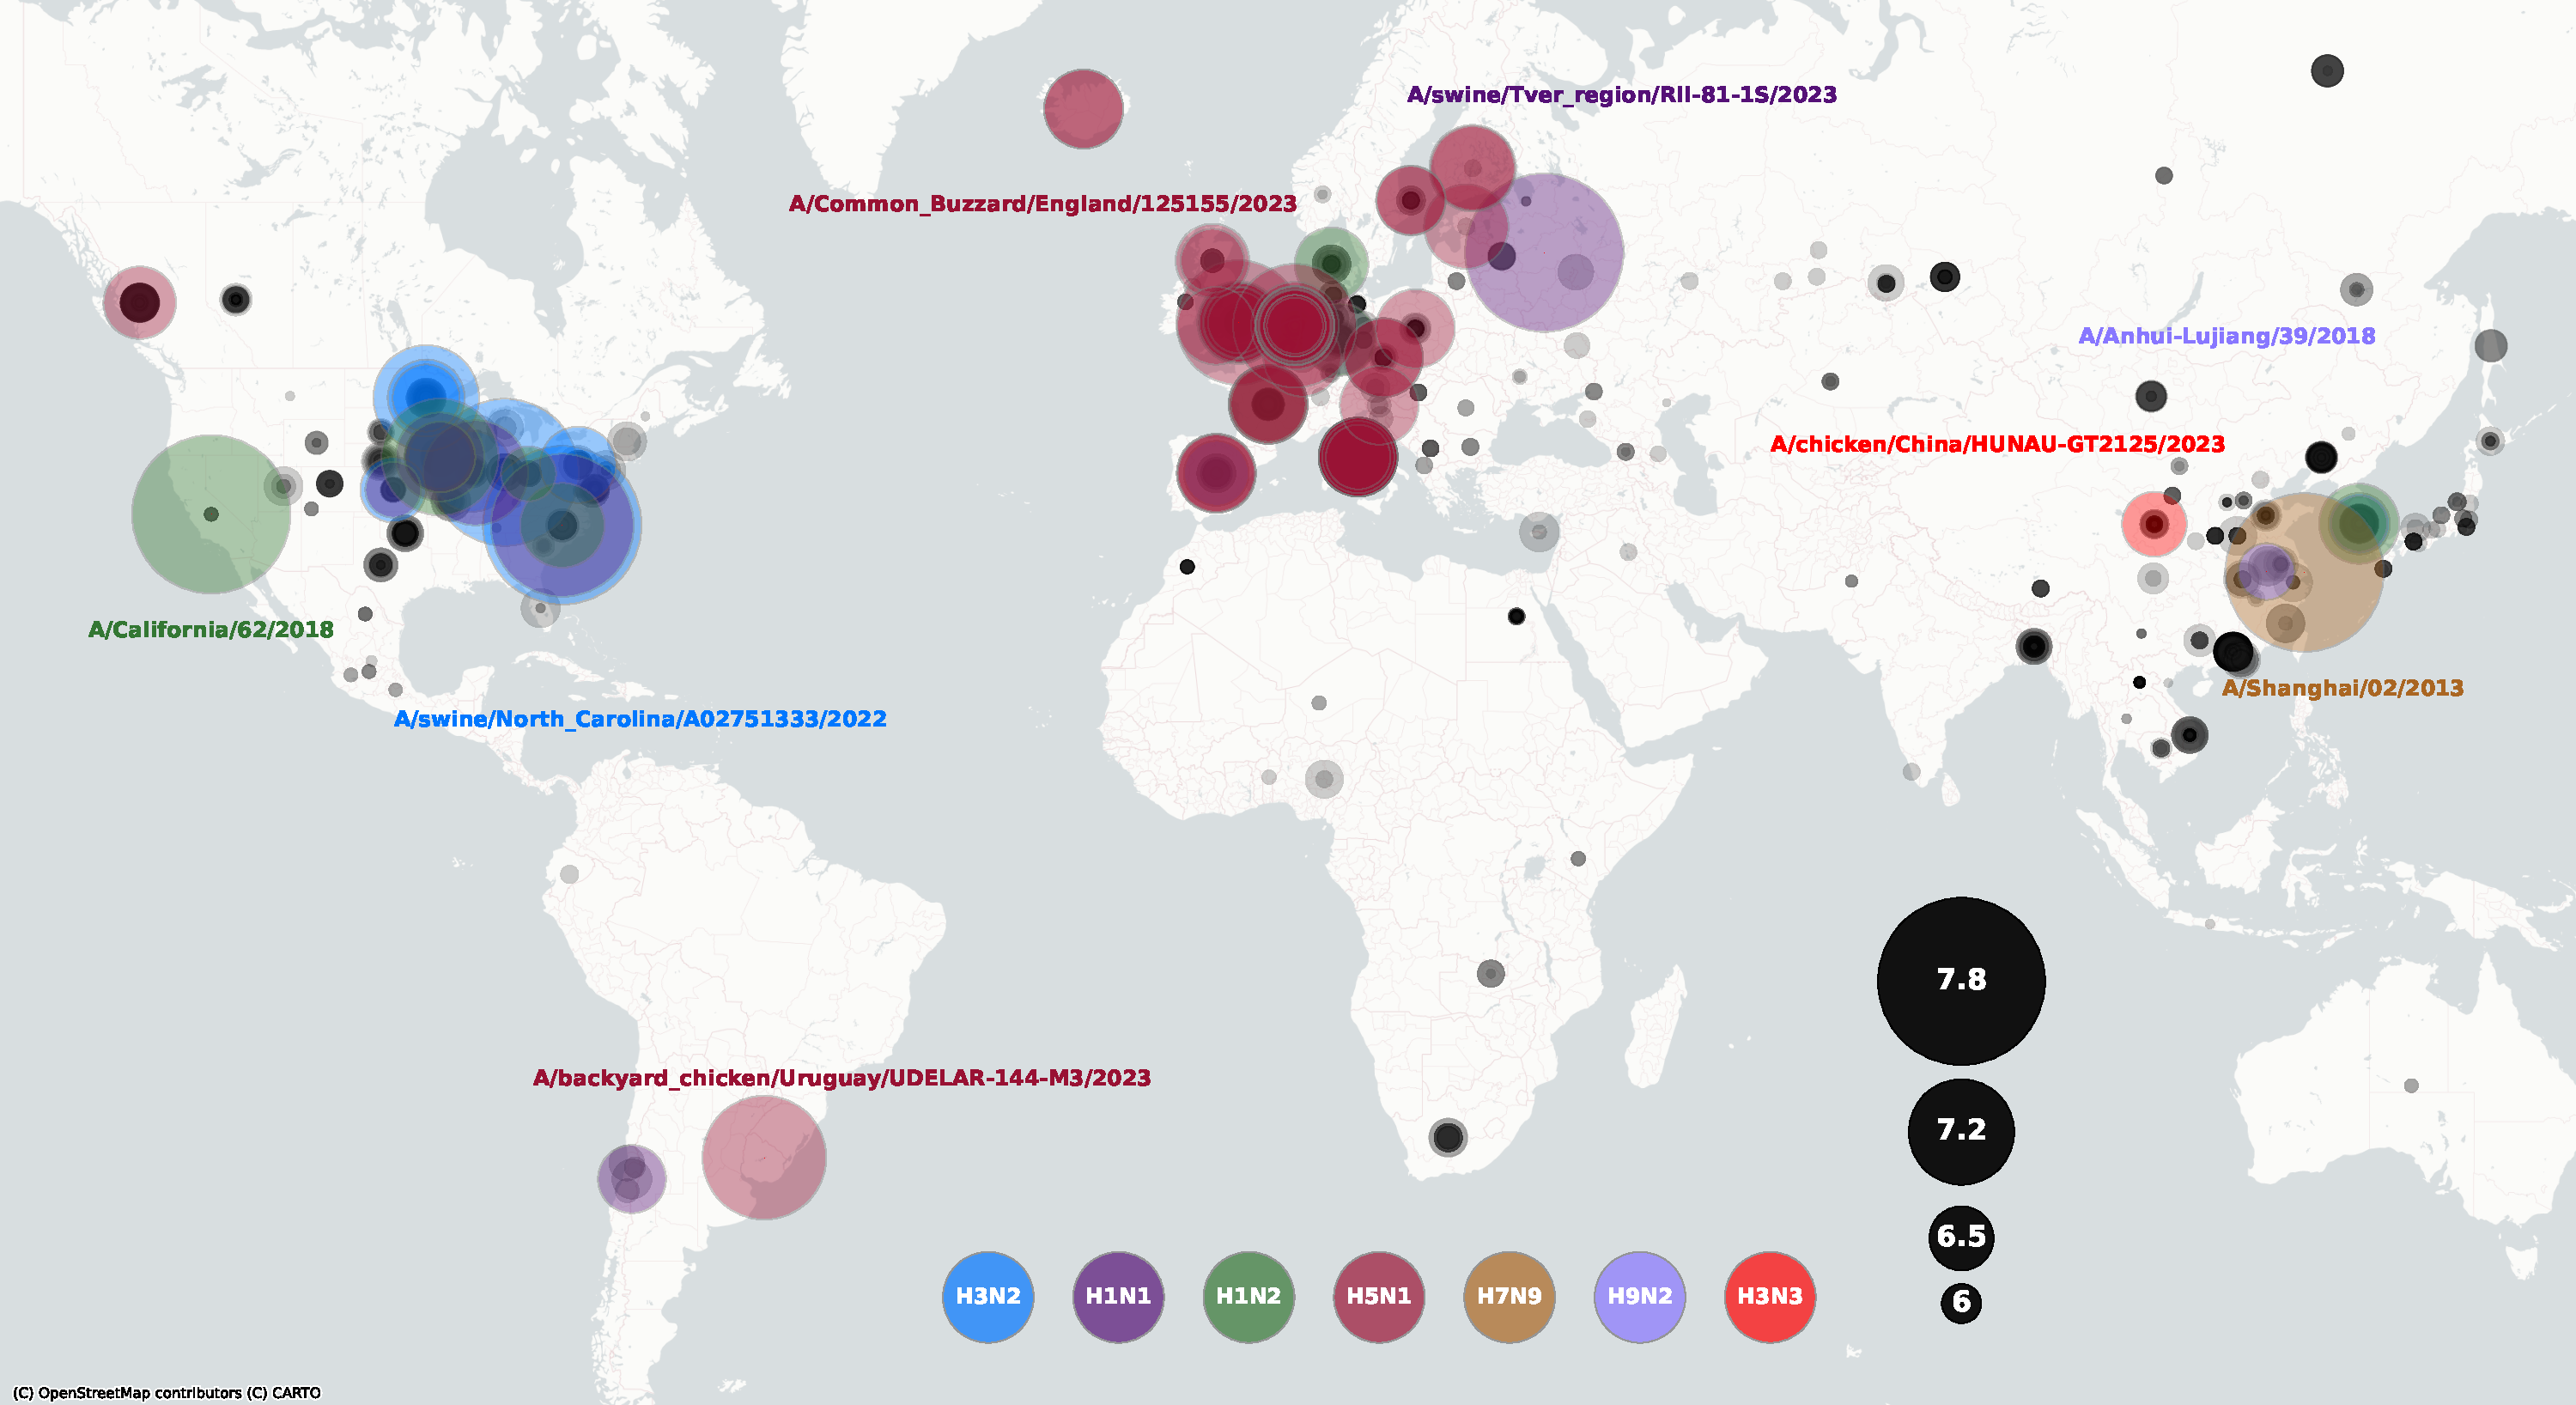
\includegraphics[width=\textwidth]{Figures/bionorad}};
\end{scope}

%7.5 7.2 6.8 <6
\def\TEXTCOLA{black!60}

\node[circle,fill=white,inner sep=1pt,text width=.185in,draw=\TEXTCOLA,label={[text=gray,xshift=.2in,align=center,font=\bf\sffamily\fontsize{7}{8}\selectfont]90:Predicted emergence  score}] (C1) at ([xshift=-1.65in,yshift=.9in]A11.center) {};
\node [anchor=west,align=left,text=\TEXTCOLA,] (LL1) at ([xshift=.1in]C1.center) {$6.8$};
\node[circle,fill=white,text width=.15in,draw=\TEXTCOLA,inner sep=1pt,,anchor=north,text=\TEXTCOLA] (C1) at ([yshift=-.1in]C1.south) {};
\node[circle,fill=white,text width=.1in,draw=\TEXTCOLA,inner sep=1pt,,anchor=north,text=\TEXTCOLA] (C1) at ([yshift=-.1in]C1.south) {};
\node[circle,fill=white,text width=.06in,inner sep=1pt,draw=\TEXTCOLA,,anchor=north,text=\TEXTCOLA] (C1) at ([yshift=-.1in]C1.south) {};
\node[circle,fill=white,inner sep=1pt,text width=.03in,draw=\TEXTCOLA,,anchor=north,text=\TEXTCOLA] (C1) at ([yshift=-.12in]C1.south) {};
\node [anchor=north,align=left,text=\TEXTCOLA] (LL1) at ([yshift=-.14in]LL1.south) {$6.5$};
\node [anchor=north,align=left,text=\TEXTCOLA] (LL1) at ([yshift=-.07in]LL1.south) {$6.1$};
\node [anchor=north,align=left,text=\TEXTCOLA] (LL1) at ([yshift=-0.06in]LL1.south) {$5.9$};
\node [anchor=north,align=left,text=\TEXTCOLA] (LL1) at ([yshift=-0.04in]LL1.south) {$5.5$};

\node[font=\sffamily\fontsize{6}{6}\selectfont,align=center,fill=Red1!80,text width=.25in,anchor=north,xshift=-0.050in,yshift=-.351in,label={[font=\bf\sffamily\fontsize{7}{8}\selectfont,
  xshift=.2in,text=gray]90:subtypes of risky Influenza Viruss}] (X1) at (C1.south) {H1N1};
\node[font=\sffamily\fontsize{6}{6}\selectfont,align=center,text=white,fill=Blue1!80,text width=.25in,anchor=north,xshift=0in,yshift=-.051in] (X2) at (X1.south) {H3N2};
\node[font=\sffamily\fontsize{6}{6}\selectfont,align=center,text=white,fill=DarkOrange1,text width=.25in,anchor=west,xshift=0.02in,yshift=0in] (X1) at (X1.east) {H9N2};
\node[font=\sffamily\fontsize{6}{6}\selectfont,align=center,fill=Green3!70,text width=.25in,anchor=north,xshift=0in,yshift=-.0501in] (X1) at (X1.south) {H7N9};

\node [text=Red1] (LD2) at ([yshift=-0.25in,xshift=-1.95in]A11.east) {};
\draw [] (LD2) node [text=DarkOrange3,fill=white,fill opacity=.2,text opacity=1,xshift=-0in,right,below,align=right,font=\bf\sffamily\fontsize{5}{5}\selectfont,xshift=-.25in] {A/mink/China/chick\_embryo/2020\\(emergence: 6.3, impact: 6.3)}  -- ++(.4in,0in) -- ++(.24in,.24in) ;


\node [text=Red1] (LD3) at ([yshift=.85in,xshift=-2.10in]A11.east) {};
\draw [] (LD3) node [text=Green3,right,above,align=center,font=\bf\sffamily\fontsize{5}{5}\selectfont,xshift=-.25in] {A/Camel/Inner\_Mongolia/XL/2020\\(emergence: 6.7, impact: 6.6)}  -- ++(.4in,0in) -- ++(.6in,-.60in) ;

% \node [text=Red1] (LD3) at ([yshift=1.15in,xshift=-1.05in]A11.east) {};
% \draw [] (LD3) node [text=Red1,right,above,align=center,font=\bf\sffamily\fontsize{5}{5}\selectfont,xshift=-.25in] {A/swine/Karaganda/04/2020\\(emergence: 6.27, impact: 6.04)}  -- ++(-.4in,0in) -- ++(-.55in,-.55in) ;

	
\node [text=Red1] (LD4) at ([yshift=-.5in,xshift=.48in]A11.west) {};
\draw [] (LD4) node [text=Red1,right,below,xshift=.45in,align=center,font=\bf\sffamily\fontsize{5}{5}\selectfont,xshift=-.25in] {A/swine/Missouri/A02524711/2020\\(emergence: 6.71, impact: 6.63)}  -- ++(-.4in,0in) -- ++(.5in,.5in) ;

	
\node [text=Red1] (LD4) at ([yshift=.5in,xshift=.8in]A11.west) {};
\draw [] (LD4) node [text=Blue1,right,above,xshift=.35in,align=center,font=\bf\sffamily\fontsize{5}{5}\selectfont,xshift=-.25in] {A/swine/Indiana/A02524710/2020\\(emergence: 6.67, impact: 6.61)}  -- ++(.3in,0in) -- ++(-.25in,-.25in) ;


\end{tikzpicture}
    };

  
\node[anchor=south west] (LA) at (A.north west) {{\Large a.} \bf Predicted emergence risk vs published IRAT scores};
%\node[anchor=south west,align=left] (LB) at ([xshift=0in]B.north west) {{\Large b.} \bf Estimating emergence};
%\node[anchor=south west] (LC) at ([xshift=.1in]C.north west) {{\Large c.} \bf Estimating  impact};
\node[anchor=south west] (LW) at ([xshift=0in]W.north west) {{\Large b.} \bf Global prediction of IRAT scored for all \infl sequences collected since 2020};


\end{tikzpicture}
  